\documentclass[10pt]{beamer}

% Tema Limpo e Profissional
\usetheme{Madrid}
\usecolortheme{whale}

% Pacotes Essenciais
\usepackage[utf8]{inputenc}
\usepackage[portuguese]{babel}
\usepackage{graphicx}
\usepackage{booktabs}
\usepackage{amsmath}
\usepackage{amssymb}
\usepackage{listings}
\usepackage{xcolor}

% Configuracoes de Codigo (Python)
\lstset{
    language=Python,
    basicstyle=\ttfamily\tiny,
    keywordstyle=\color{blue},
    stringstyle=\color{red},
    commentstyle=\color{green!60!black},
    breaklines=true,
    showstringspaces=false
}

% Metadados com Prevencao de Avisos de Metadados PDF
\title[ADS - Aula 14 (P2)]{Função de Verossimilhança}
\subtitle{Máxima Verossimilhança para Modelos Discretos e Contínuos}
\author[ADS - IFCE]{Tecnologia em Análise e Desenvolvimento de Sistemas\texorpdfstring{\\ \small{Ciência de Dados / Estatística Computacional}}{}}
\institute[IFCE]{Instituto Federal do Ceará -- Campus Tauá \\ Tecnologia em Análise e Desenvolvimento de Sistemas}
\date{\today}

\begin{document}

\begin{frame}
    \titlepage
\end{frame}

\begin{frame}{Sumário da Aula}
    \tableofcontents
\end{frame}

% Blocos Modulares de Slides
\section{Função de Verossimilhança de Bernoulli}

\begin{frame}{O que é Verossimilhança?}
    \begin{itemize}
        \item Até o momento, avaliamos o ajuste de modelos por meio de critérios puramente geométricos (como a minimização do Erro Quadrático Médio).
        \item A \textbf{Função de Verossimilhança} ($L$) nos permite estimar parâmetros de modelos sob uma perspectiva probabilística.
        \item \textbf{Cenário Dedutivo (Probabilidade):}
        \begin{itemize}
            \item Os parâmetros populacionais $\theta$ são conhecidos (ex: moeda justa, $\theta = 0.5$).
            \item Queremos calcular a chance de observar um determinado conjunto de dados.
        \end{itemize}
        \item \textbf{Cenário Indutivo (Inferência/Verossimilhança):}
        \begin{itemize}
            \item Os dados amostrais já foram coletados e estão fixos.
            \item Queremos avaliar a plausibilidade de diferentes valores do parâmetro $\theta$.
        \end{itemize}
    \end{itemize}
\end{frame}

\begin{frame}{O Modelo Discreto: Ensaios de Bernoulli}
    \begin{itemize}
        \item Considere uma sequência de lançamentos de moedas independentes.
        \item Cada lançamento $X_i \in \{0, 1\}$ segue uma distribuição de Bernoulli com $P(X_i = 1) = \theta$.
        \item A Função de Massa de Probabilidade ($PMF$) de Bernoulli é escrita como:
        $$P(X_i = x_i) = \theta^{x_i} (1 - \theta)^{1 - x_i}$$
        \item Assumindo observações independentes e identicamente distribuídas, a \textbf{Função de Verossimilhança} de uma amostra de tamanho $N$ é o produto das PMFs individuais:
        $$L(\theta) = \prod_{i=1}^N P(X_i = x_i) = \prod_{i=1}^N \theta^{x_i} (1 - \theta)^{1 - x_i}$$
        $$L(\theta) = \theta^{\sum_{i=1}^N x_i} (1 - \theta)^{N - \sum_{i=1}^N x_i}$$
    \end{itemize}
\end{frame}

\begin{frame}{Visualizando a Verossimilhança de Bernoulli}
    \begin{columns}
        \begin{column}{0.5\textwidth}
            \textbf{Experimento Prático:}
            \begin{itemize}
                \item Jogamos uma moeda $N = 13$ vezes e observamos $4$ caras ($1$) e $9$ coroas ($0$).
                \item A função de verossimilhança é:
                $$L(\theta) = \theta^4 (1 - \theta)^9$$
                \item \textbf{Ponto de Máximo:}
                Graficamente, a plausibilidade é maximizada em $\theta \approx 0.3077$.
                \item \textbf{Desafio Numérico:}
                Os valores de $L(\theta)$ são muito pequenos (na ordem de $10^{-4}$).
            \end{itemize}
        \end{column}
        \begin{column}{0.5\textwidth}
            \centering
            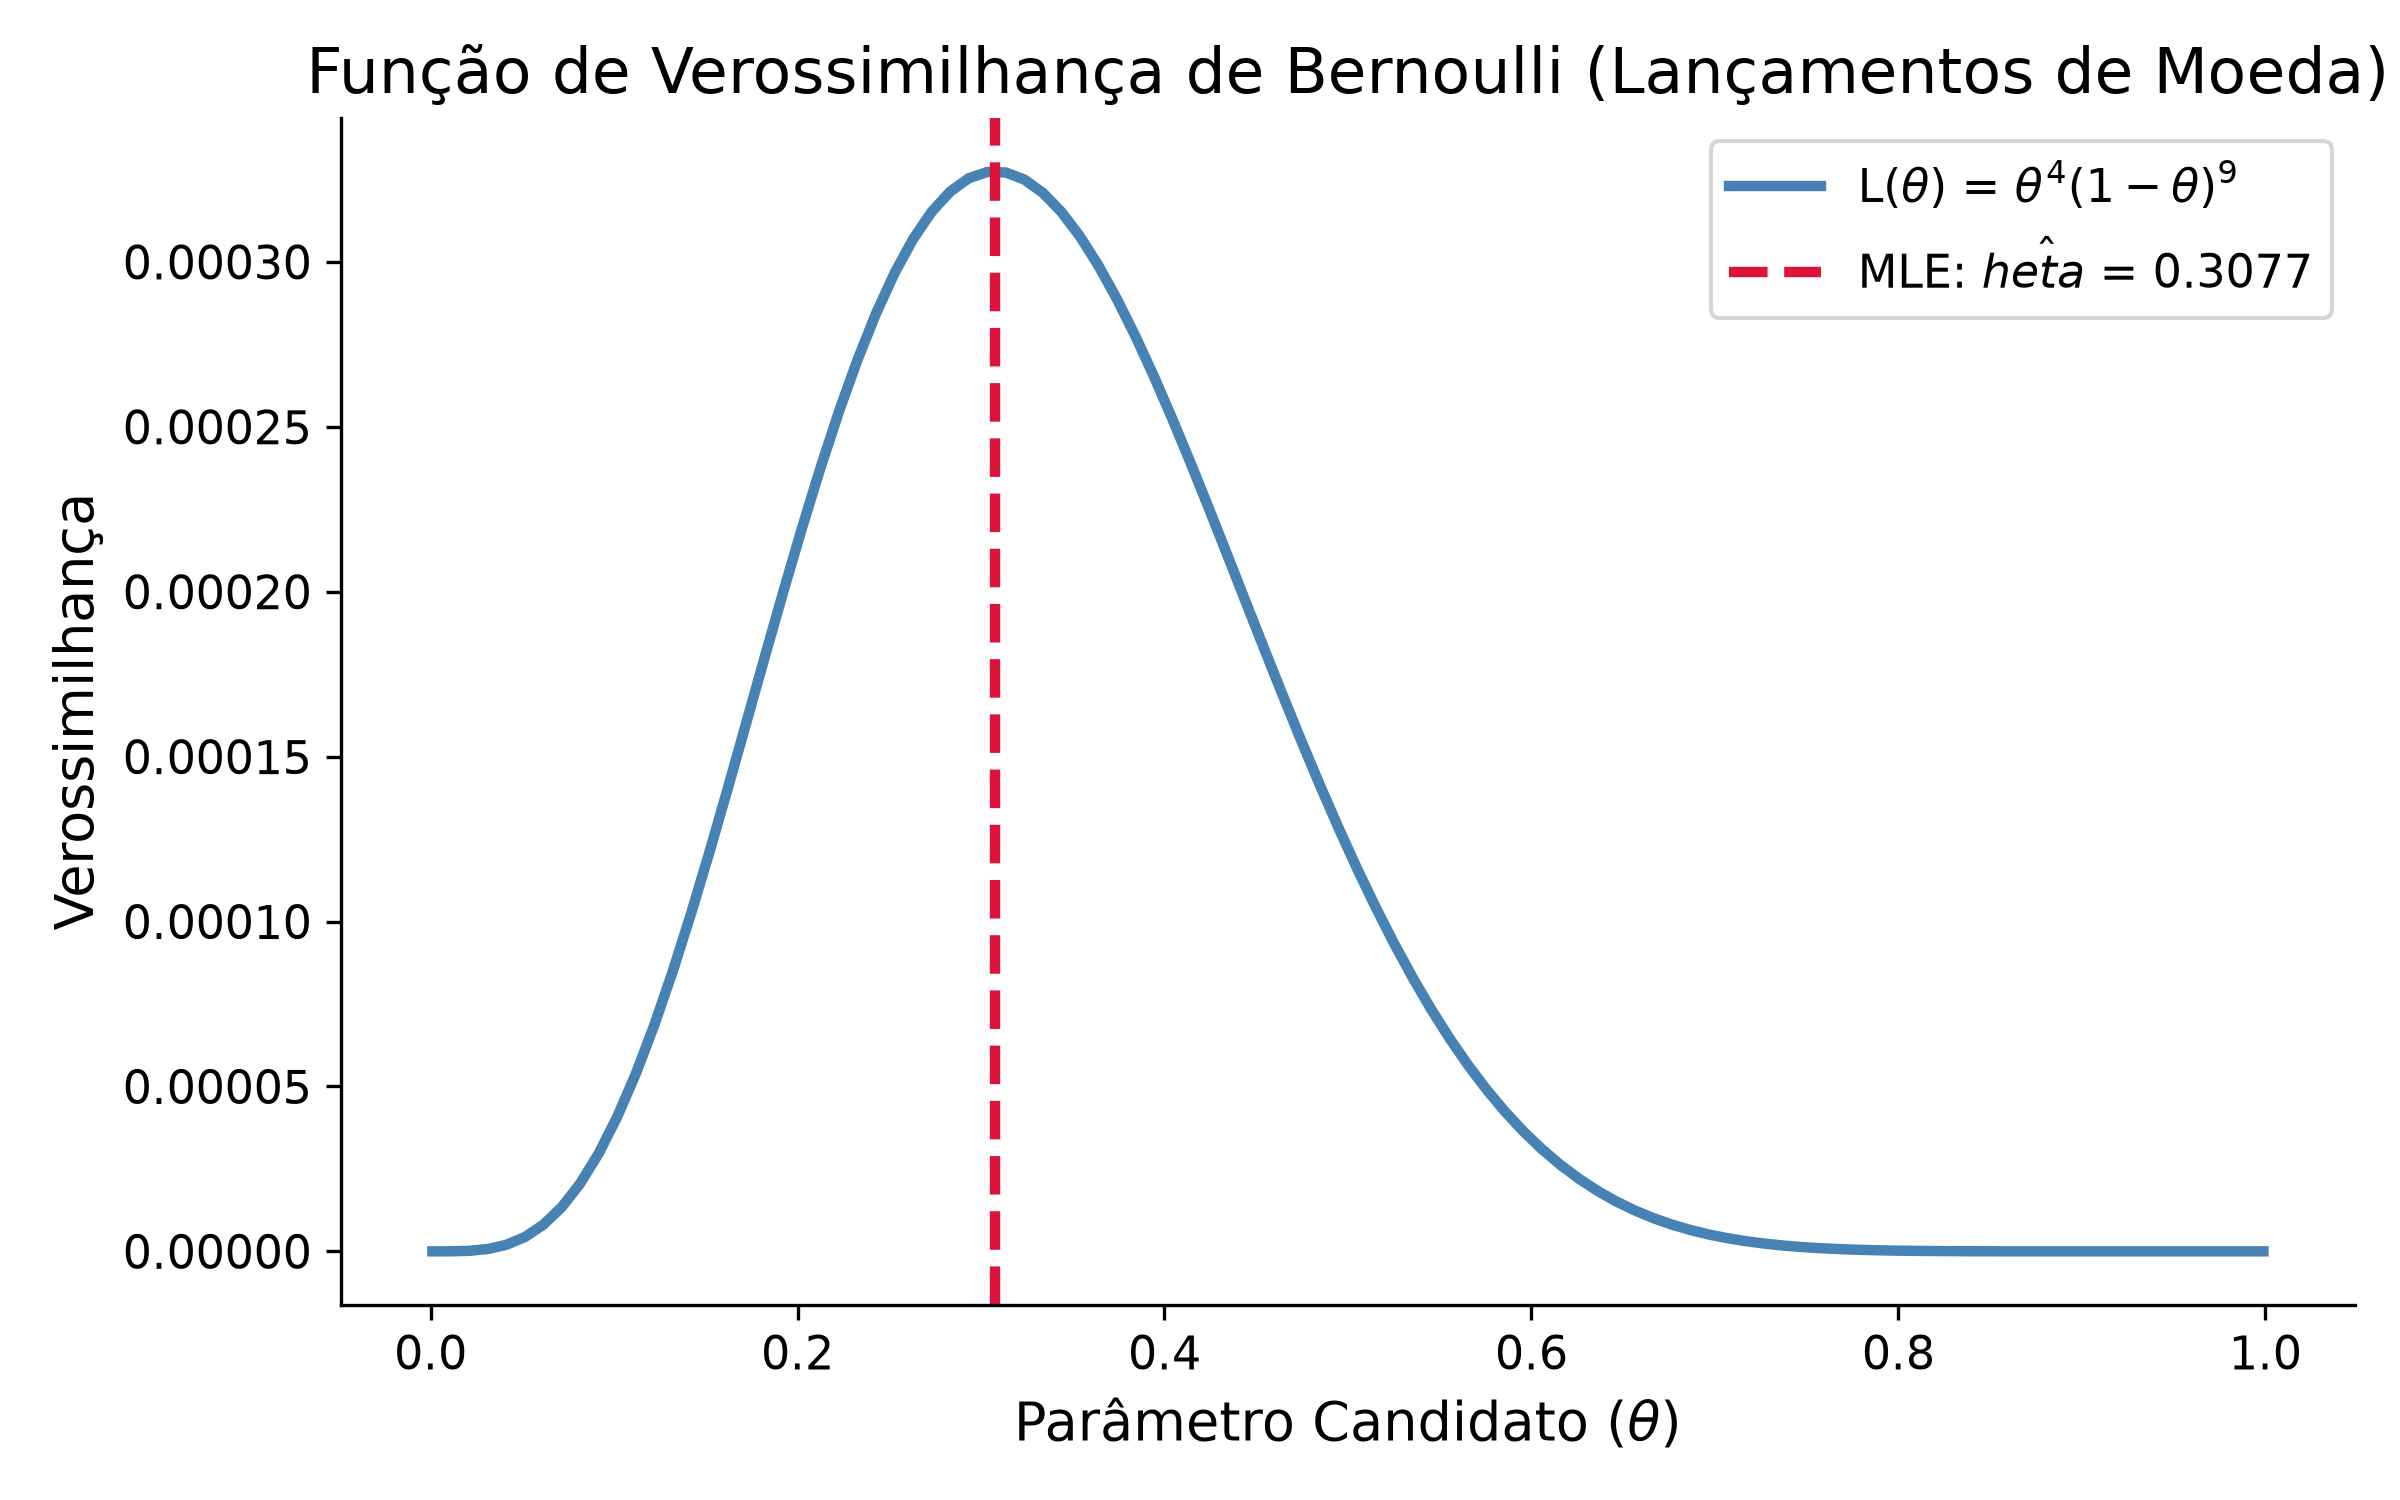
\includegraphics[width=\textwidth]{verossimilhanca_bernoulli.png}
        \end{column}
    \end{columns}
\end{frame}

\begin{frame}{A Escala de Log-Verossimilhança}
    \begin{itemize}
        \item Para computadores, multiplicar dezenas ou centenas de probabilidades menores que 1 gera \textbf{subfluxo numérico} (underflow), onde o produto é arredondado para zero.
        \item Aplicando a função de logaritmo natural ($\ln$) na verossimilhança, convertemos produtos em somatórios:
        $$\ln L(\theta) = \ln \left( \prod_{i=1}^N P(X_i = x_i) \right) = \sum_{i=1}^N \ln P(X_i = x_i)$$
        \item Como a função $\ln(y)$ é estritamente crescente, o valor de $\theta$ que maximiza a log-verossimilhança é o mesmo que maximiza a verossimilhança original.
        \item Para o caso de Bernoulli:
        $$\ln L(\theta) = \left( \sum_{i=1}^N x_i \right) \ln \theta + \left( N - \sum_{i=1}^N x_i \right) \ln(1 - \theta)$$
    \end{itemize}
\end{frame}

\begin{frame}{Visualizando a Log-Verossimilhança}
    \begin{columns}
        \begin{column}{0.5\textwidth}
            \textbf{Escala de Log-Verossimilhança:}
            \begin{itemize}
                \item O valor máximo da curva ocorre no mesmo ponto:
                $$\theta \approx 0.3077$$
                \item A escala no eixo vertical agora varia em valores negativos mais estáveis (não decai para zero).
                \item Facilita a modelagem computacional e a obtenção das derivadas.
            \end{itemize}
        \end{column}
        \begin{column}{0.5\textwidth}
            \centering
            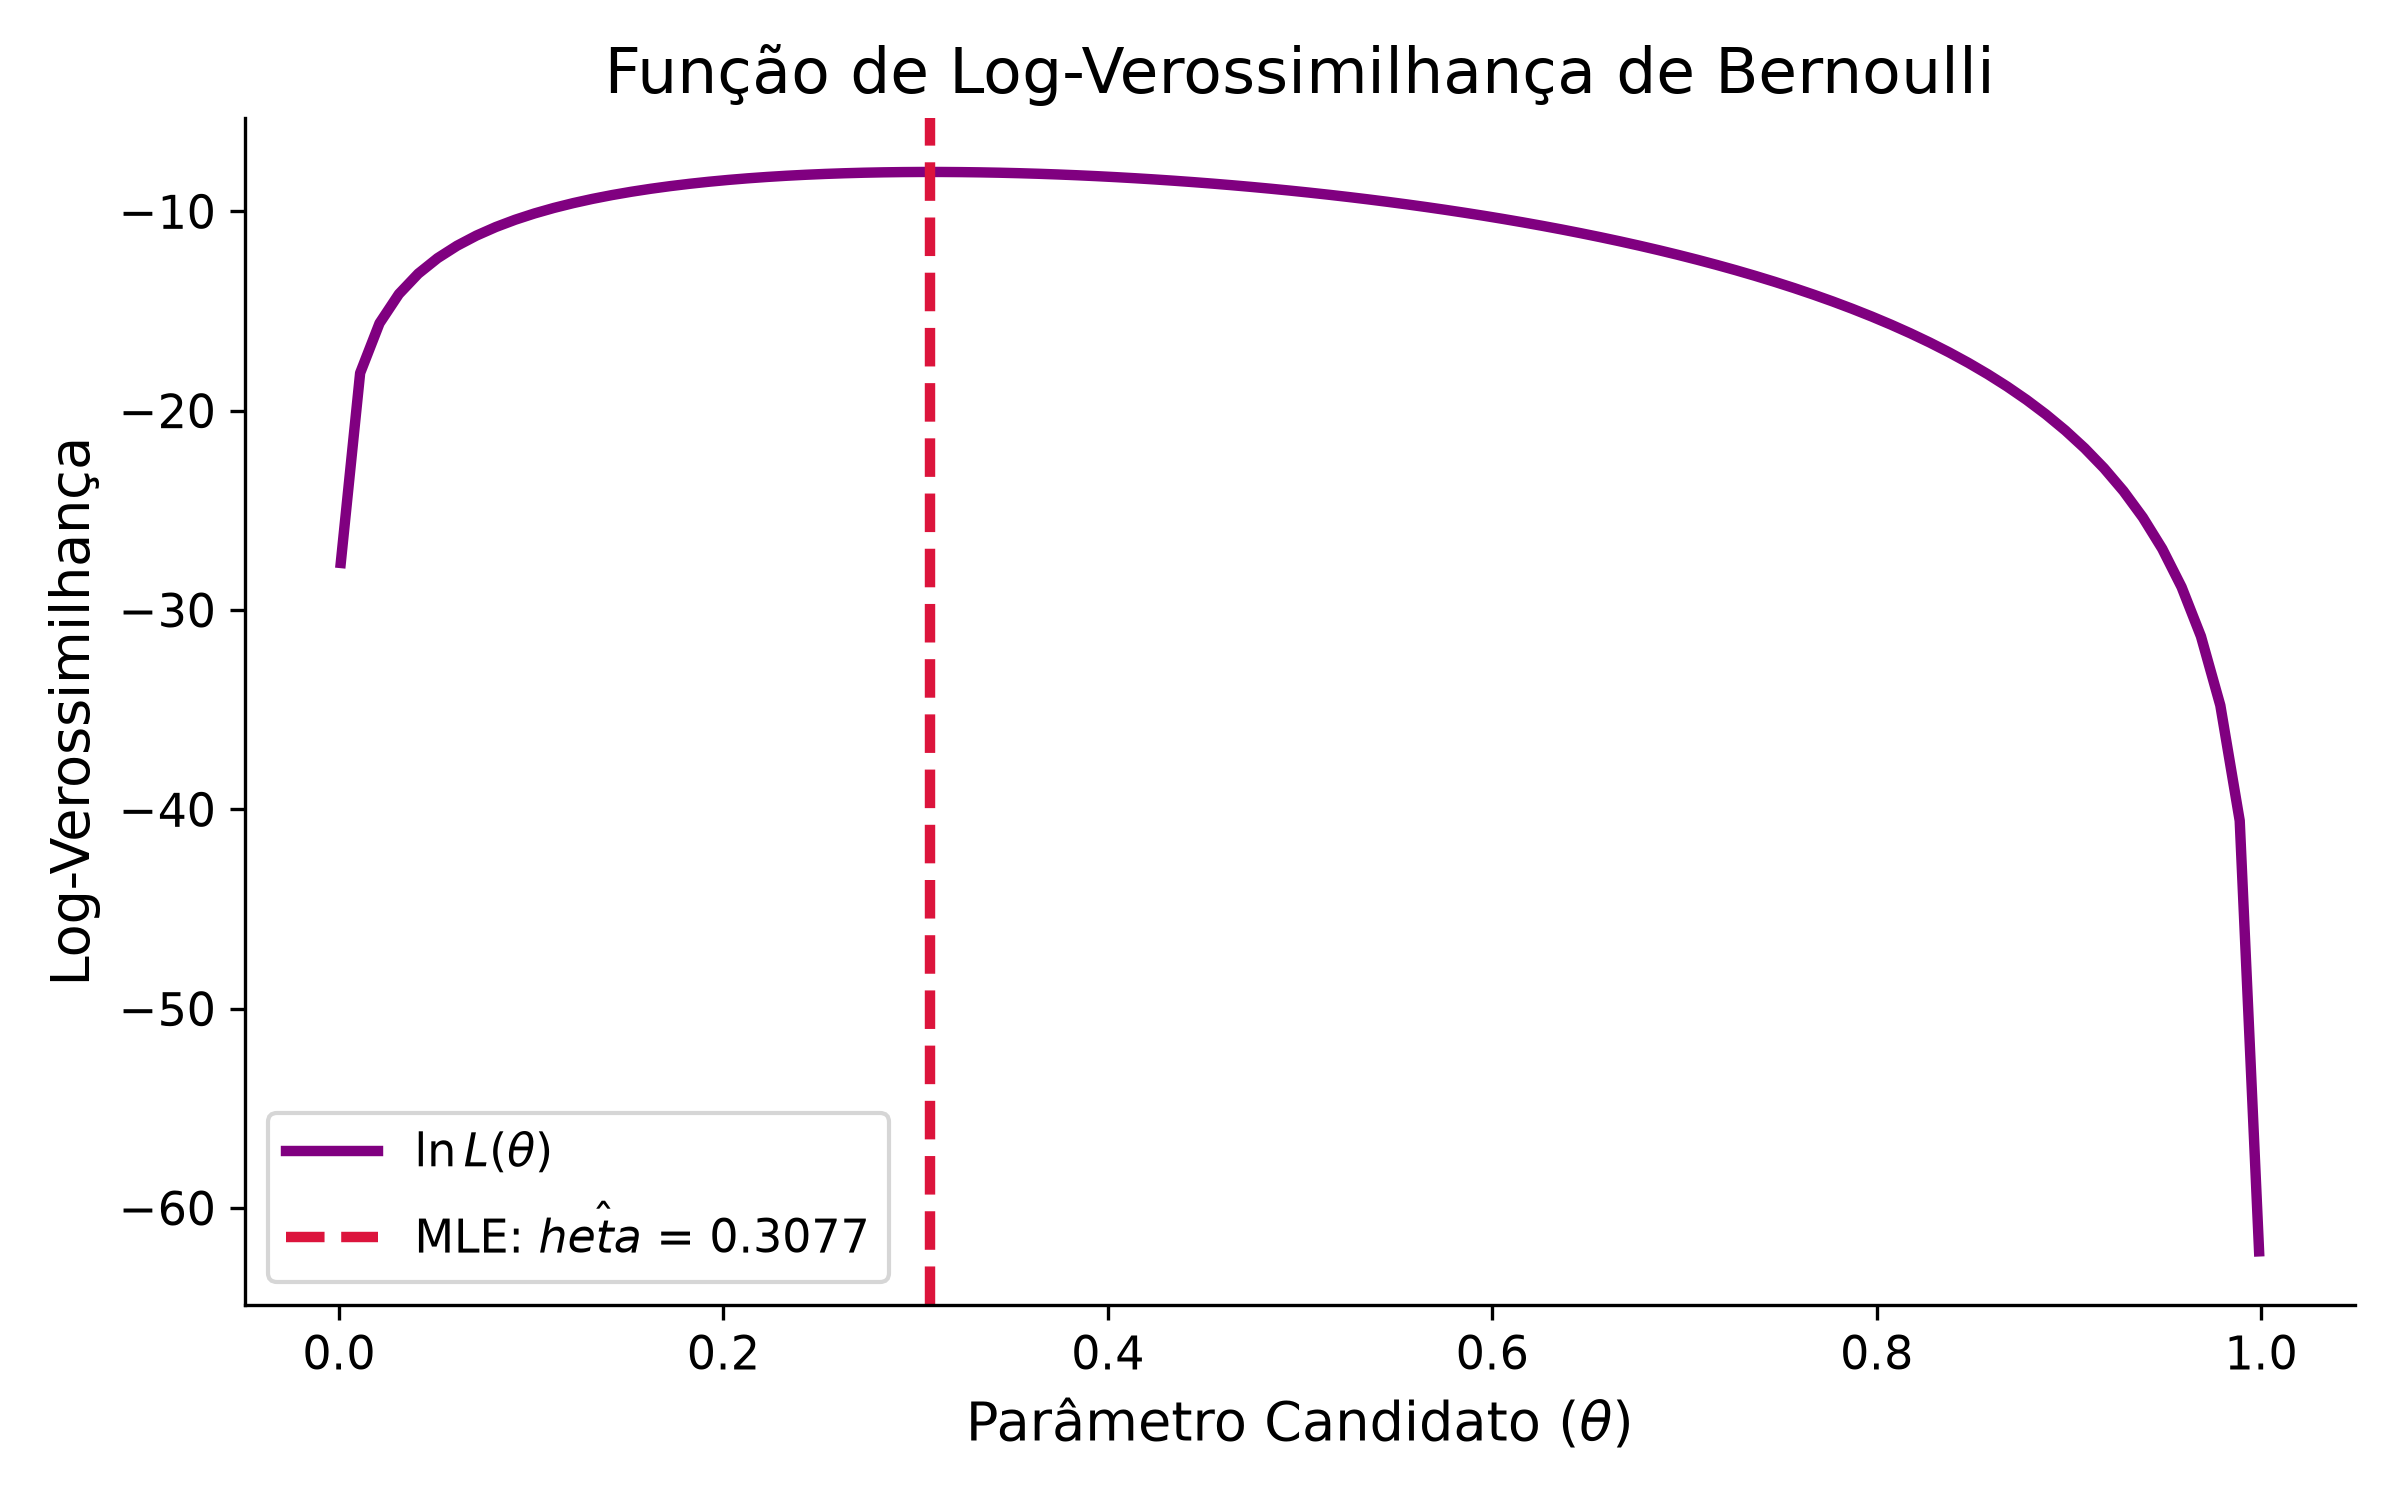
\includegraphics[width=\textwidth]{log_verossimilhanca_bernoulli.png}
        \end{column}
    \end{columns}
\end{frame}

\begin{frame}{Exemplo Pareado: Solução Analítica}
    \begin{itemize}
        \item Queremos encontrar o valor de $\theta$ que maximiza a log-verossimilhança:
        $$\ln L(\theta) = (\sum x_i) \ln \theta + (N - \sum x_i) \ln(1 - \theta)$$
        \item Derivamos com relação ao parâmetro $\theta$ e igualamos a zero para achar o ponto crítico:
        $$\frac{d \ln L(\theta)}{d\theta} = \frac{\sum x_i}{\theta} - \frac{N - \sum x_i}{1 - \theta} = 0$$
        $$\frac{\sum x_i}{\theta} = \frac{N - \sum x_i}{1 - \theta} \implies (1 - \theta) \sum x_i = \theta (N - \sum x_i)$$
        $$\sum x_i - \theta \sum x_i = \theta N - \theta \sum x_i \implies \hat{\theta}_{MLE} = \frac{\sum x_i}{N}$$
        \item \textbf{Conclusão:} A Estimativa de Máxima Verossimilhança ($\hat{\theta}_{MLE}$) para a proporção é a própria proporção amostral dos dados.
    \end{itemize}
\end{frame}

\begin{frame}[fragile]{Exemplo Pareado: Implementação em Python}
    \begin{block}{Calculando a Log-Verossimilhança de Bernoulli}
\begin{lstlisting}
import numpy as np

# Dados do experimento (4 caras, 9 coroas)
dados = np.array([1, 1, 1, 1, 0, 0, 0, 0, 0, 0, 0, 0, 0])
N = len(dados)
sucessos = np.sum(dados)
fracassos = N - sucessos

# Proporcao empirica (MLE)
theta_otimo = sucessos / N
print(f"MLE de theta: {theta_otimo:.4f}") # Saida: 0.3077

# Funcao de log-verossimilhanca
def log_verossimilhanca(theta, k, n):
    return k * np.log(theta) + (n - k) * np.log(1 - theta)

# Testando valores candidatos de theta
for theta in [0.1, 0.3077, 0.5, 0.8]:
    ll = log_verossimilhanca(theta, sucessos, N)
    print(f"Theta: {theta:.4f} | Log-Verossimilhanca: {ll:.4f}")
\end{lstlisting}
    \end{block}
\end{frame}

\section{Verossimilhança Gaussiana e Atividade}

\begin{frame}{Modelagem de Dados Contínuos: A Normal}
    \begin{itemize}
        \item Para dados contínuos, a verossimilhança é formulada utilizando a \textbf{Função de Densidade de Probabilidade} ($PDF$).
        \item Assumimos que a nossa amostra segue uma distribuição Normal $N(\mu, \sigma^2)$:
        $$f(x_i | \mu, \sigma^2) = \frac{1}{\sqrt{2\pi\sigma^2}} \exp\left(-\frac{(x_i - \mu)^2}{2\sigma^2}\right)$$
        \item Onde $\mu$ é a \textbf{Média Populacional} e $\sigma^2$ é a \textbf{Variância Populacional}.
        \item A verossimilhança conjunta para $N$ observações independentes é dada pelo produtório:
        $$L(\mu, \sigma^2) = \prod_{i=1}^N f(x_i | \mu, \sigma^2) = \prod_{i=1}^N \frac{1}{\sqrt{2\pi\sigma^2}} \exp\left(-\frac{(x_i - \mu)^2}{2\sigma^2}\right)$$
        $$L(\mu, \sigma^2) = \left(2\pi\sigma^2\right)^{-N/2} \exp\left(-\frac{1}{2\sigma^2} \sum_{i=1}^N (x_i - \mu)^2\right)$$
    \end{itemize}
\end{frame}

\begin{frame}{A Log-Verossimilhança Gaussiana}
    \begin{itemize}
        \item Aplicando a transformação logarítmica natural ($\ln$) à verossimilhança Normal:
        $$\ln L(\mu, \sigma^2) = \ln \left[ \left(2\pi\sigma^2\right)^{-N/2} \exp\left(-\frac{1}{2\sigma^2} \sum_{i=1}^N (x_i - \mu)^2\right) \right]$$
        $$\ln L(\mu, \sigma^2) = -\frac{N}{2} \ln(2\pi\sigma^2) - \frac{1}{2\sigma^2} \sum_{i=1}^N (x_i - \mu)^2$$
        \item \textbf{A Conexão com Mínimos Quadrados:}
        \begin{itemize}
            \item Para maximizar a verossimilhança com relação à média $\mu$, a primeira parcela é constante.
            \item Portanto, devemos **maximizar** a segunda parcela, o que equivale a **minimizar** o somatório $\sum_{i=1}^N (x_i - \mu)^2$.
            \item Esse somatório é exatamente a soma dos erros quadráticos!
        \end{itemize}
    \end{itemize}
\end{frame}

\begin{frame}{Estimadores de Máxima Verossimilhança}
    \begin{itemize}
        \item Derivando a log-verossimilhança com relação a $\mu$ e igualando a zero:
        $$\frac{\partial \ln L}{\partial \mu} = \frac{1}{\sigma^2} \sum_{i=1}^N (x_i - \mu) = 0 \implies \hat{\mu}_{MLE} = \frac{1}{N}\sum_{i=1}^N x_i = \bar{X}$$
        \item Derivando com relação a $\sigma^2$ e igualando a zero:
        $$\frac{\partial \ln L}{\partial (\sigma^2)} = -\frac{N}{2\sigma^2} + \frac{1}{2(\sigma^2)^2} \sum_{i=1}^N (x_i - \mu)^2 = 0 \implies \hat{\sigma}^2_{MLE} = \frac{1}{N}\sum_{i=1}^N (x_i - \bar{X})^2$$
        \item \textbf{Nota Importante:}
        O estimador de máxima verossimilhança da variância divide por $N$ e não por $N - 1$. Isso o torna ligeiramente viesado para pequenas amostras.
    \end{itemize}
\end{frame}

\begin{frame}{Visualizando a Log-Verossimilhança Normal}
    \begin{columns}
        \begin{column}{0.5\textwidth}
            \textbf{Análise da Média Amostral:}
            \begin{itemize}
                \item Utilizando a amostra de 170 medições de sala.
                \item Mantemos o desvio padrão constante no seu valor ótimo $\hat{\sigma} \approx 16.6020$.
                \item Avaliamos diferentes médias candidatas $\mu$.
                \item A log-verossimilhança Gaussiana atinge o seu valor máximo exatamente em:
                $$\hat{\mu}_{MLE} = 46.5412$$
            \end{itemize}
        \end{column}
        \begin{column}{0.5\textwidth}
            \centering
            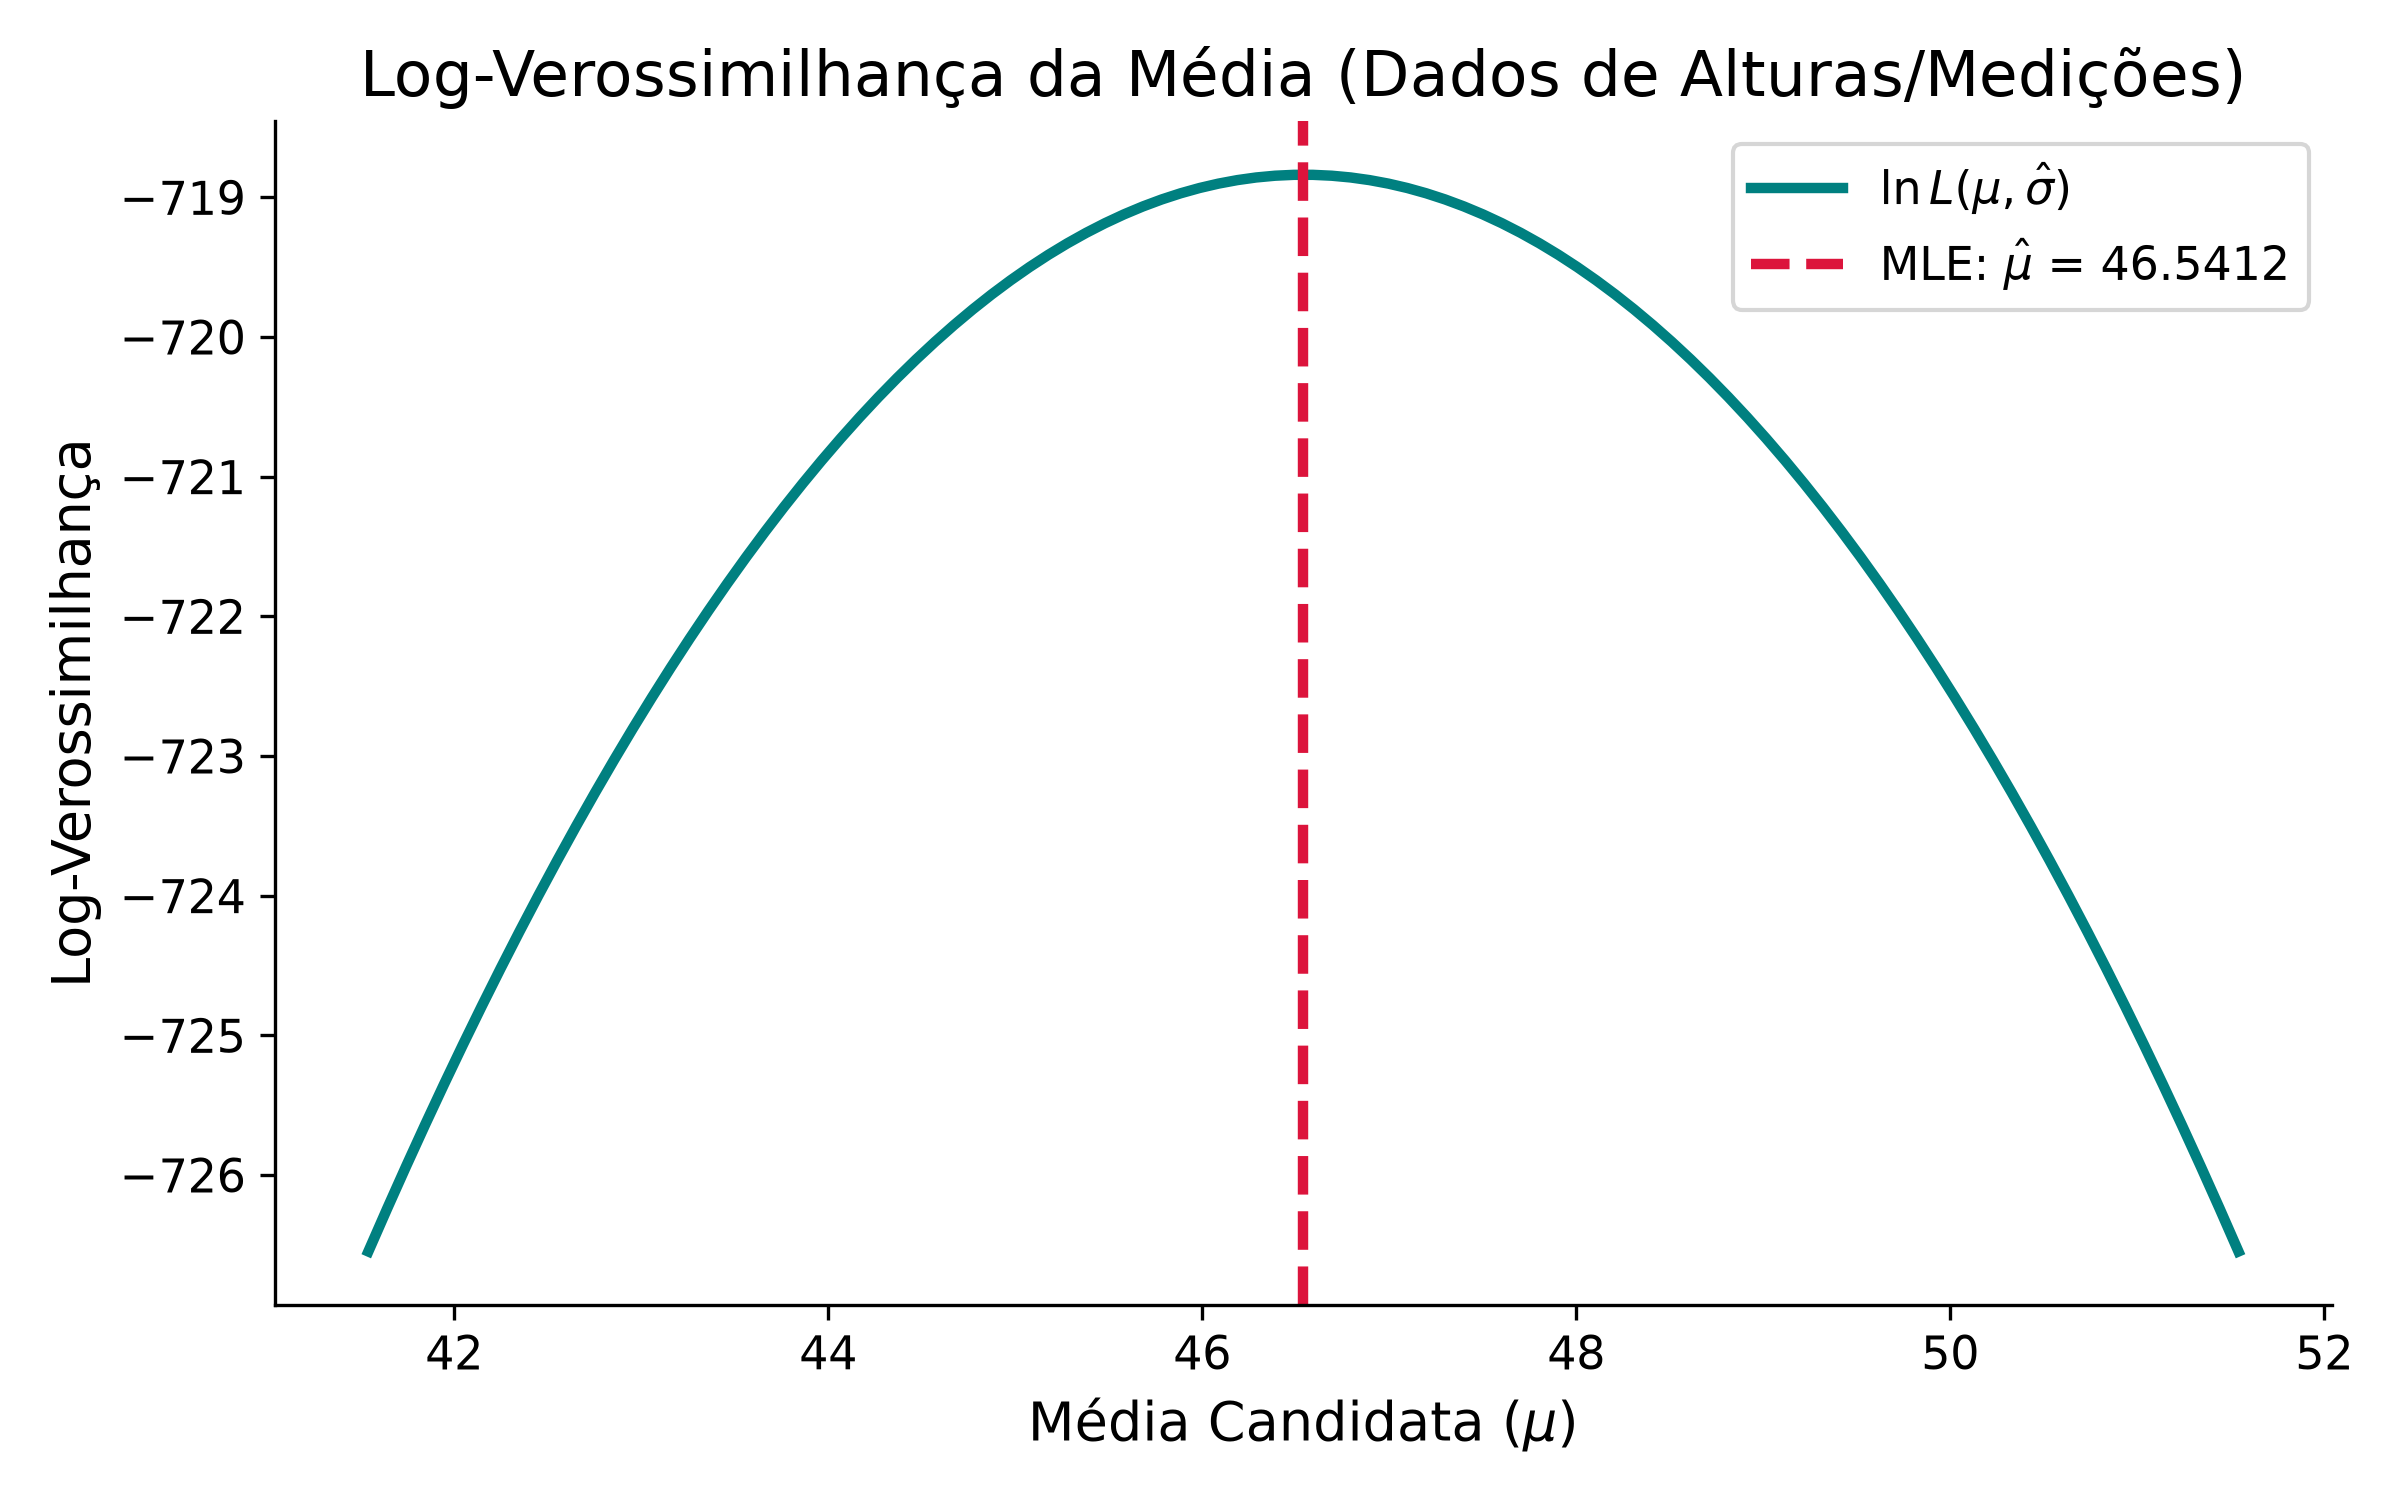
\includegraphics[width=\textwidth]{log_verossimilhanca_normal_mu.png}
        \end{column}
    \end{columns}
\end{frame}

\begin{frame}[fragile]{Exemplo Pareado: Avaliação Gaussiana}
    \begin{block}{Implementando a Log-Verossimilhança Normal em Python}
\begin{lstlisting}
import numpy as np
import scipy.stats as ss

# Amostra de medicoes
dados = np.array([41, 27, 33, 58, 24, 65, 48, 72, 36, 29, 54, 67, 21])

# Estimativas pontuais amostrais
media_amostral = np.mean(dados)
std_amostral = np.std(dados) # MLE divide por N

print(f"Media amostral: {media_amostral:.4f}")

# Funcao de log-verossimilhanca Normal usando scipy
def log_verossimilhanca_normal(dados, mu, sigma):
    pdf_valores = ss.norm.pdf(dados, loc=mu, scale=sigma)
    return np.sum(np.log(pdf_valores))

# Avaliando medias candidatas
for mu_cand in [30.0, media_amostral, 60.0]:
    ll = log_verossimilhanca_normal(dados, mu_cand, std_amostral)
    print(f"Mu candidato: {mu_cand:.4f} | Log-Verossimilhanca: {ll:.4f}")
\end{lstlisting}
    \end{block}
\end{frame}

\begin{frame}{Atividade Prática de Laboratório}
    \begin{itemize}
        \item Abra um Jupyter Notebook no ambiente do curso.
        \item \textbf{Tarefa 1 (Simulação de Moeda):}
        \begin{itemize}
            \item Simule 100 lançamentos de moeda com probabilidade $\theta = 0.65$.
            \item Implemente a função de log-verossimilhança de Bernoulli.
            \item Plote a curva de log-verossimilhança para um grid de valores candidatos e identifique o ponto de máximo.
        \end{itemize}
        \item \textbf{Tarefa 2 (Dados Gaussianos):}
        \begin{itemize}
            \item Simule 50 observações normais com média $\mu = 30$ e desvio padrão $\sigma = 5$.
            \item Crie uma função para calcular a log-verossimilhança normal.
            \item Mantenha $\sigma = 5.0$ fixo e avalie a plausibilidade para médias de 20 a 40.
            \item Verifique se o máximo numérico coincide com a média amostral observada.
        \end{itemize}
    \end{itemize}
\end{frame}


\end{document}
